\documentclass{beamer}
\usetheme{Dresden}
\usecolortheme{beaver}
\usepackage{fontspec}

\title{EpNet Day lectures\\
    Acerbi et al : The Logic of Fashion Cycles
}
\author{Simon Carrignon}
\date{20-11-2015}
\begin{document}
\begin{frame}
    
\maketitle
\end{frame}
\section{Intro}
\begin{frame}{Introduction}
    Aim of the article :

    \begin{itemize}
	\item Propose a new model of cultural evolution (\emph{preference model})
	\item compare this model to :
	    \begin{itemize}
		\item Neutral Model (random copy)
		\item Status Model (copy of the people with higher social status)
	    \end{itemize}
	\item Evaluate the three models against real data
    \end{itemize}
\end{frame}
\section{Author's model}
\begin{frame}
    \begin{block}{General idea of the study}
	Preference for a cultural traits is itself a cultural trait: analyse the co-evolution of those two kind traits :
	\begin{itemize}
	    \item a cultural trait
	    \item a preference to this cultural trait
	\end{itemize}
    \end{block}
\end{frame}
\begin{frame}{One cultural trait}
    They first create a model with one cultural trait and a preference for that traits, so 4 types of individuals :
    \begin{enumerate}
	\item $0$ no trait, no preference for it
	\item $T$ the trait but no preference
	\item $P$ the prefenrence but not possessing the trait
	\item $PT$ posses the trait and a preference for it.
    \end{enumerate}
    Based on that agent interact and when meet on \emph{observer} copies a \emph{model}.
\end{frame}
\begin{frame}{Transmission probability}
    \begin{figure}
	\center
	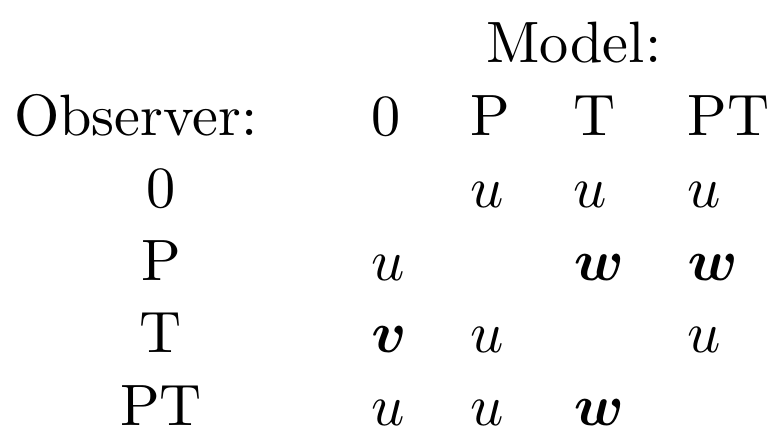
\includegraphics[width=5cm]{table_s1.png}
	\caption{From SI Acerbi et al 2012}
    \end{figure}

    assumption :
    \begin{description}
	\item[$v>u$]someone with preference for a traits is more likely to lose it and 
	\item[$w>u$]someone with a preference for a traits is more likely to adopt it
    \end{description}
    %\begin{description}
    %    \item[w] it the observer as a preference ($P$ agent) for the traits and the model has the traits ($T$ or $PT$ model) or if the  (w>u)
    %    \item[v]if the observer
    %    \item[u]else
    
\end{frame}
\end{document}


